In the following sub-appendices, we describe various methods used to select and validate the data, models, and approaches presented in the main text. 
In Appendix~\ref{appendix:model_comparison_mass} and Appendix~\ref{appendix:model_comparison_spins} we discuss the process for selecting the fiducial mass and spin models, respectively, under the \parametric and present results from other models which were under consideration.
Appendix~\ref{appendix:model_comparison_effective_spins} describes how the specific convergence cut biases the inferred effective spin distribution. 
In Appendix~\ref{appendix:non_parameteric_comparison}, we compare various types of methods for the \nonparametric, which were presented in Appendix~\ref{appendix:non_parametric_models_summary}.
Appendix~\ref{appendix:FGMC_rates} gives compact object merger rates when sub-threshold triggers are considered, i.e., using a lower~\ac{FAR} threshold. 
Finally, Appendix~\ref{appendix:supplementary_correlations} provides supplementary results for population-level correlations between masses, spins, and redshifts.

\begin{deluxetable}{lcc}
\tablecaption{Bayes factor comparison of selected models from the mass model comparison study.}
\tablehead{
    \colhead{Model} & \colhead{Abbreviation} & \colhead{$\log_{10}\mathcal{B}$}
}
\label{tab:model_comparison_mass}
\startdata
\BrokenPLTwoPeaks $\bigstar$ & \BPTP & $0$ \\
\tableline
\textsc{Broken Power Law + 1 Peak} & \BPOP & $\BBHMassModelBayesFactors[pl2pk1]$ \\
\textsc{Broken Power Law + 3 Peaks} & \BPHP & $\BBHMassModelBayesFactors[pl2pk3]$ \\
\textsc{Power Law + Peak} & \PP & $\BBHMassModelBayesFactors[plp]$ \\
\enddata
\end{deluxetable}

\begin{figure*}[t]
	\centering
	  \includegraphics[width=\textwidth]{figures/fig_primary_mass_appendix.pdf}
	  \caption{Inferred mass distributions of various \parametrics compared to the fiducial mass model \BrokenPLTwoPeaks (gray shaded) and 
	  the \BSpline model (black dashed). The fiducial model from \gwtcthree, \PLPeak, is shown in orange, a broken power law with a single peak in blue, and a broken power law with three peaks in pink.}
	  \label{fig:mass_model_comp_1}
  \end{figure*}

\subsection{Model Comparison Study: Mass}\label{appendix:model_comparison_mass}

\begin{figure}
	\centering
	  \includegraphics[width=120mm]{figures/fig_primary_mass_default_modes.pdf}
	  \caption{Differential merger rate as a function of primary mass (evaluated at $z=0.2$) of the two different modes recovered by the \BrokenPLTwoPeaks model. The orange shaded region shows the 90\% credible interval for the dominant mode ($\BBHMassModelBayesFactors[default_dominant_mode]\%$ of posterior), reflecting a distinct peak at $35 \,\Msun$, and the purple shaded region shows the $90\%$ credible interval for the subdominant mode ($\BBHMassModelBayesFactors[default_subdominant_mode] \%$ of posterior), reflecting a broken power law morphology without a distinct $35 \,\Msun$ peak. The black dashed lines show the $90\%$ credible bounds of the \textsc{Broken Power Law + 1 Peak} model for comparison. The inset figure shows the joint posterior of the peak mean $\mu_2$ and width $\sigma_2$ for each mode. The vertical grey shaded region indicates the $90\%$ credible interval of the sum $\mu_2 + \sigma_2$, which is consistent between both modes.}
	  \label{fig:primary_mass_modes}
  \end{figure}

The fiducial mass model is a \parametric that is intended to provide a minimal but accurate description of the data with a parametrization that is more readily interpretable than the \nonparametrics.  
Table \ref{tab:model_comparison_mass} shows the Bayes factors between models with a different number of features and our fiducial model \BrokenPLTwoPeaks. 
We also compare to our previous fiducial model from \citet{KAGRA:2021duu}, the \PLPeak model. 
In Figure \ref{fig:mass_model_comp_1}, we see that \PLPeak infers the peak component at $35\Msun$, as in \citet{KAGRA:2021duu}, but a broken power law plus 1 peak (\BPOP) model infers the peak component at $10\Msun$ and the power law break at $35\Msun$. 
In Table \ref{tab:model_comparison_mass}, we see that all models that include a broken power law are strongly favored over the \PLPeak model. 

However, among models with a broken power law, the Bayes factors do not show strong support for one model over another. 
Bayes factors are a useful model comparison metric when they are decisive (e.g., requiring a broken power law), however minor preferences should not be taken too seriously: $\log_{10}$ Bayes factors less than $\sim 0.5$ should be considered ambiguous \citep{Jeffreys:1939xee}.
In addition, for the set of hierarchical models we consider here, the priors are neither physically motivated nor can they be made consistent between models. 
Bayes factors are prior-dependent, which means the value of the Bayes factor itself is subjective. 
Therefore, among the models not decisively ruled out by Bayes factor, we select the most interpretable extension of the \PLPeak model that probes features shared among all of the \nonparametrics shown in Figure \ref{fig:bbh_mass_non_parametrics}. 
The \BrokenPLTwoPeaks model best fit these criteria.

In \gwtcthree, the \PLPeak model identified an overdensity in the merger rate at $m_1 =$ \muTOT relative to a global power law. 
Evidence for this feature first appeared in \citet{LIGOScientific:2018jsj} and was strengthened in \citet{LIGOScientific:2020kqk} and \citet{KAGRA:2021duu}. 
As mentioned in Section \ref{subsec:bbh_masses}, this feature at $35\Msun$ may be an overdensity relative to an underlying mass continuum or could mark the onset of a decline in the merger rate. 
In addition to the Bayes factor comparison shown in Table \ref{tab:model_comparison_mass}, this ambiguity is also present in the \BrokenPLTwoPeaks posterior, which includes two posterior modes (identified with a k-means clustering algorithm) that correspond to two different morphologies, shown in Figure \ref{fig:primary_mass_modes}. 
The dominant mode is correlated with a narrower ($\sigma_2 = \CIPlusMinus{\DefaultBBHDominantMode[sigpp_2]} \,\Msun$) peak at $\mu_2 = \CIPlusMinus{\DefaultBBHDominantMode[mpp_2]} \,\Msun$ and accounts for $\BBHMassModelBayesFactors[default_dominant_mode] \%$ of the posterior volume, while the subdominant mode is correlated with a wider ($\sigma_2 = \CIPlusMinus{\DefaultBBHSubdominantMode[sigpp_2]} \,\Msun$) peak at $\mu_2 = \CIPlusMinus{\DefaultBBHSubdominantMode[mpp_2]} \,\Msun$ and accounts for $\BBHMassModelBayesFactors[default_subdominant_mode]\%$ of the posterior volume. 
This latter mode has a morphology nearly identical to the inferred \BPOP distribution (see Figure \ref{fig:primary_mass_modes}). 
The inflection point of the Gaussian, $\mu_2 + \sigma_2 = \CIPlusMinus{\defaultbbh[mu_plus_sig]} \,\Msun$, is consistent between both modes, which indicates that the right half of the Gaussian must fall below the power law to match the declining rate in this region (the gray vertical shaded region in Figure \ref{fig:primary_mass_modes}).

The power law indices, $\alpha_1$ and $\alpha_2$ are not correlated with the two modes present in the \BPTP posterior, though the measured slope of the mass distribution between $18{-}19 \,\Msun$ is not equivalent to $\alpha_1$ in the subdominant mode. 
In this mode, the slope (calculated by finite difference) is $\CIPlusMinus{\DefaultBBHSubdominantMode[mass_1][powerlaw_slope_18-19]}$, which includes more support for negative values compared to the inferred power law index, $\alpha_1 = \CIPlusMinus{\DefaultBBHSubdominantMode[alpha_1]}$. 
We infer the power law break location at $m_\text{break} = \CIPlusMinus{\defaultbbh[break_mass]} \,\Msun$. 
The \BPOP model, which does not include a second Gaussian component, measures the break location much more precisely at $m_\text{break} = \CIPlusMinus{\PowerLawTwoPeakOneBBH[break_mass]} \,\Msun$. 
The uncertainty in the \BPTP power law break is due to the presence of the second Gaussian component, which likely obscures the break most of the time. 
Because the peak is narrower in the dominant \BPTP mode, one might expect the break location to be better constrained in this mode; however, this is not the case. 
The break location does not appear to be correlated with either mode.

\ExtendedBrokenPLTwoPeaks also possesses the two modes seen in \BrokenPLTwoPeaks, but with some key differences. 
Like \BrokenPLTwoPeaks, the two modes are distinguished by the inferred location of the second Gaussian component. 
The dominant mode in \ExtendedBrokenPLTwoPeaks places the second Gaussian component at ${\sim} 35 \,\Msun$. 
Unlike \BrokenPLTwoPeaks, this mode accounts for $\VaryingBetaQsDominantModeBetaDiffPerc[dom_posterior_fraction] \%$ of the posterior. 
Additionally, the correlation between primary mass and mass ratio allowed by \ExtendedBrokenPLTwoPeaks breaks the degeneracy in the inferred power law break location seen in the two modes of \BrokenPLTwoPeaks. 
The power law break location is uninformed in the dominant mode (because it is obscured by the second Gaussian component), but is measured near ${\sim} 35 \,\Msun$ in the subdominant mode. 
The mass ratio power law index of the second Gaussian component in the dominant mode is $\beta_q^{\rm peak2} = \CIPlusMinus{\VaryingBetaQsDominantMode[param][beta_q_high_mass_peak]}$, which is what we report in the main text (Section \ref{subsec:bbh_masses}). 
In contrast, the subdominant mode measures $\beta_q^{\rm peak2}$ as being strictly negative, and as in \BrokenPLTwoPeaks, prefers the location of the second Gaussian component to be less than $30 \,\Msun$. 
The mass ratio power law index of the continuum mass component, $\beta_q^{\rm BP}$ is strictly positive in this mode. 
Given these findings, the second Gaussian mass component in the dominant mode and the continuum mass component in the subdominant mode of \ExtendedBrokenPLTwoPeaks appear to be describing the same feature, which is that ${\sim}35 \,\Msun$ BHs are more likely to pair with other BHs of equal mass relative to the rest of the continuum. 
This result is most clearly described by the dominant mode, which is why (in addition to it accounting for $\VaryingBetaQsDominantModeBetaDiffPerc[dom_posterior_fraction] \%$ of the posterior) we quote the dominant mode results in the main text.

\subsection{Model Comparison Study: Spin Magnitudes and Tilt Angles}\label{appendix:model_comparison_spins}


\begin{deluxetable}{llllc}
\tablecaption{
    Comparison of different parametric models for spin magnitudes $\chi_i$ and tilt angles $\cos\theta_i$.
}
\tablehead{
    \colhead{$\chi_i$ model} & \colhead{} & \colhead{$\cos\theta_i$ model} & \colhead{} & \colhead{$\log_{10}\mathcal{B}$}
}
\label{tab:modelComparisonSpins}
\startdata
Truncated Gaussian $\bigstar$ & IID & Isotropic + Truncated Gaussian & NID & $\spinModelComparisonLogTenBayesFactors[MagTruncnormIidTiltIsotropicTruncnormNid][log10_bayes_factor_over_new_default]$ \\
Constrained Beta & IID & Isotropic + Aligned Gaussian & NID & $\spinModelComparisonLogTenBayesFactors[MagBetaConstrainedIidTiltIsotropicAlignedNid][log10_bayes_factor_over_new_default]$ \\
\tableline
Constrained Beta & IID & Isotropic + Truncated Gaussian & NID & $\spinModelComparisonLogTenBayesFactors[MagBetaConstrainedIidTiltIsotropicTruncnormNid][log10_bayes_factor_over_new_default]$ \\
Unconstrained Beta & IID & Isotropic + Truncated Gaussian & NID & $\spinModelComparisonLogTenBayesFactors[MagBetaUnconstrainedIidTiltIsotropicTruncnormNid][log10_bayes_factor_over_new_default]$ \\
Truncated Gaussian & IID & Isotropic + Aligned Gaussian & NID & $\spinModelComparisonLogTenBayesFactors[MagTruncnormIidTiltIsotropicAlignedNid][log10_bayes_factor_over_new_default]$ \\
\tableline
Truncated Gaussian & IND & Isotropic + Truncated Gaussian & NID & $\spinModelComparisonLogTenBayesFactors[MagTruncnormIndTiltIsotropicTruncnormNid][log10_bayes_factor_over_new_default]$ \\
Truncated Gaussian & IID & Isotropic + Truncated Gaussian & NND & $\spinModelComparisonLogTenBayesFactors[MagTruncnormIidTiltIsotropicTruncnormNnd][log10_bayes_factor_over_new_default]$\\
Truncated Gaussian & IND & Isotropic + Truncated Gaussian& NND & $\spinModelComparisonLogTenBayesFactors[MagTruncnormIndTiltIsotropicTruncnormNnd][log10_bayes_factor_over_new_default]$ \\
\enddata
\tablecomments{The first row is the Default model for \gwtcfour (\default), while the second is the Default that was used for \gwtcthree and earlier~\citep{LIGOScientific:2018jsj,LIGOScientific:2020kqk,KAGRA:2021duu,Talbot:2017yur}.
The third through final are other models explored. All log Bayes factors ($\log_{10}\mathcal{B}$) are with respect to the first row.}
\end{deluxetable}

We consider two additional spin magnitude models beyond the \default~model from Section~\ref{subsubsec:bbh_spin_mag_and_tilts}: the Constrained Beta and Unconstrained Beta models, both defined by Equation~\eqref{eqn:beta_distribution}. 
We also consider one additional spin tilt model, the Isotropic + Aligned Gaussian, which fixes $\mu_t = 1$ in the \default~model and served as the {\sc Default} in \gwtcthree~\citep{Talbot:2017yur,KAGRA:2021duu}.
The first five rows of Table~\ref{tab:modelComparisonSpins} give the log Bayes factors between these models.
Within the \default~model, we also test whether the primary and secondary spins are identically and independently distributed (see Appendix~\ref{appendix:iid}), with log Bayes factors given in the bottom three rows of Table~\ref{tab:modelComparisonSpins}.
The \default~model with IID spin magnitudes and NID spin tilts performs the best, and is adopted as the default component spin model in the main text.

Figure \ref{fig:spin_mags_tilts_comparison_cornerplot} shows posteriors for the magnitude and tilt hyperparameters assuming that $\chi_i$ and $\cos\theta_i$ are both identically distributed (gray) versus both non-identically distributed (blue and red). 
The primary and secondary spins have consistent hyperparameter distributions.
Assuming identical distribution makes the hyperparameters more-precisely constrained---yielding tighter 90\% bands on the resultant population distributions---but does not affect the overall shape of the distributions. 
The only difference of note is that $\chi_2$ has less support for a small $\mu_\chi$ than $\chi_1$, potentially hinting at more highly spinning secondary BHs on a population level. 

%
\begin{figure*}
	\centering
	\includegraphics[width=0.8\linewidth]{figures/spins/spin_model_comparison_cornerplot.pdf}
	\caption{Distribution of \default~hyperparameters for the primary \ac{BH} (blue) and secondary \ac{BH} (red) when neither magnitudes nor tilts are assumed identical (last row of Table~\ref{tab:modelComparisonSpins}), compared to when they are both assumed identical (gray, first row of Table~\ref{tab:modelComparisonSpins}).
	The contours of the two dimensional distributions mark the 50th and 90th percentiles.}
	\label{fig:spin_mags_tilts_comparison_cornerplot}
  \end{figure*}
%

\subsection{Dependence of the Effective Spin Distribution on the Likelihood Variance Cut}\label{appendix:model_comparison_effective_spins}

We next investigate the effect of the likelihood variance threshold (see Appendix~\ref{sec:likelihood-estimator-variance}) on our \parametricAdj effective spin results. 
To ensure that posteriors generated using Monte Carlo estimation are trustworthy, i.e., the likelihood estimate is converged, we enforce that all hyperparameter samples yield a log-likelihood variance ${\sigma^2}_{\ln\cal \hat L} < 1$ for all analyses presented in the main text~\citep{Talbot:2023pex}.
In \gwtcthree, however, a different quantity was used to assess the Monte Carlo uncertainty: the effective number of independent samples, $N_{\rm eff}$~\citep{Farr:2019rap}. 
It was there imposed that $N_{\rm eff}$ be greater than $4 N_{\rm events}$ for the sensitivity injections used in Equation~\eqref{eq:selection_efficiency} and greater than 10 for every event in the catalog of CBCs. 
This $N_{\rm eff}$ cut is generally less stringent than the approach taken for \gwtcfour. 
The $\chip$ distribution is sensitive to which method is used to cut out samples.

For the most direct comparison to \gwtcthree, we here use the \effectiveSpinModel model.
Figure~\ref{fig:effective_spins_comparison_cornerplot} shows the posteriors for the \effectiveSpinModel parameters where the ${\sigma^2}_{\ln\cal \hat L}$ (purple) versus  $N_{\rm eff}$ (green) cuts are done on the \gwtcfour results. 
The LVK \gwtcthree results (with the $N_{\rm eff}$ cut) are shown in comparison (black). 
Figure~\ref{fig:effective_spins_comparison_dists} shows the resultant marginal and joint $\chieff$--$\chip$ population distributions. 
There are three main differences between the results with the two cuts on \gwtcfour data: 
\begin{enumerate}
	\item The ${\sigma^2}_{\ln\cal \hat L}$ cut yields a $\mu_{\rm p}$ posterior which is constrained away from zero, while the the $N_{\rm eff}$ cut does not.
	\item The $N_{\rm eff}$ cut allows for wider $\chip$ distributions (larger $\sigma_{\rm p}$) than the ${\sigma^2}_{\ln\cal \hat L}$ cut. 
	\item Under the $N_{\rm eff}$ cut, $\chieff$ and $\chip$ are preferentially positively correlated, while under the ${\sigma^2}_{\ln\cal \hat L}$ cut we remain agnostic, with preference for small-to-zero correlation.
\end{enumerate}
Thus, the claims that the $\chip$ distribution does not peak at zero, and that the data prefer $\chieff$ and $\chip$ being uncorrelated at the population level, are not necessarily astrophysical in origin.
Rather, they are driven by regions of the parameter-space that our events and sensitivity injections allow us reliably probe with Monte Carlo likelihood estimators. 

The particular sensitivity of the $\chip$ distribution to these cuts can be at-least partly attributed to the use of a uniform and isotropic spin prior in \gwtcfour~parameter estimation, which induces a $\chip$ prior that goes to $0$ at $\chip = 0,1$.
Thus, Equation~\eqref{eq:hierarchical_likelihood} is prone to yield a small $N_{\rm eff}$ and/or large ${\sigma^2}_{\ln\cal \hat L}$ when $\chip$ is near-minimal or near-maximal.
Using alternative spin priors in parameter estimation could aid in getting more effective samples at small $\chip$, improving our ability to probe the presence or absence of negligibly precessing \acp{BH} at the population level.
The Monte Carlo uncertainty from working with a finite number of samples to estimate the likelihood will only grow more problematic as the number of observed \acp{CBC} increases~\citep{Talbot:2023pex}; development of mitigation techniques is an area of active research~\citep[e.g.,][]{Gerosa:2020pgy,Rinaldi:2021bhm,Talbot:2020oeu,Callister:2022qwb, Talbot:2023pex, Leyde:2023iof,Hussain:2024qzl,Callister:2024qyq,Lorenzo-Medina:2024opt,Mancarella:2025uat}.

%
\begin{figure*}
	\centering
	\includegraphics[width=\linewidth]{figures/spins/chi_eff_chi_p_model_comparison_cornerplot.pdf}
	\caption{
	Posterior for the \effectiveSpinModel model hyperparameters, as defined in Table~\ref{tab:effectiveSpinPriors}, for \gwtcfour under two methods of cutting out samples that may lead to an unconverged likelihood.
	Posteriors excluding samples with a substantially large log-likelhood variance (${\sigma^2}_{\ln\cal \hat L}$ cut) are shown in purple; those excluding samples with a substantially small number of effective samples ($N_{\rm eff}$ cut) are in green.
	In black are the \gwtcthree results with the $N_{\rm eff}$ cut for comparison.
	The $\chieff$ hyperparameters are not affected by the cuts, while the $\chip$ and joint-distribution hyperparameters are.
	The contours of the two dimensional distributions mark the 50th and 90th percentiles.}
	\label{fig:effective_spins_comparison_cornerplot}
  \end{figure*}
%

%
\begin{figure*}
	\centering
	\includegraphics[width=\linewidth]{figures/spins/chi_eff_chi_p_model_comparison_dists.pdf}
	\caption{
	Marginal and joint $\chieff$ and $\chip$ distributions under the \effectiveSpinModel model using two methods of cutting out hyperparameter samples that may lead to an unconverged likelihood (see Figure~\ref{fig:effective_spins_comparison_cornerplot}).
	The marginal distributions show the median (solid line) and 90\% credible interval on the probability density for each population distribution (shaded).
	The joint distribution is the \ac{PPD} with contours marking the 50th and 90th quantiles.}
	\label{fig:effective_spins_comparison_dists}
  \end{figure*}
%


\subsection{Comparison of Weakly Modeled Approach Results}\label{appendix:non_parameteric_comparison}


\begin{figure*}[t]
	\centering
	  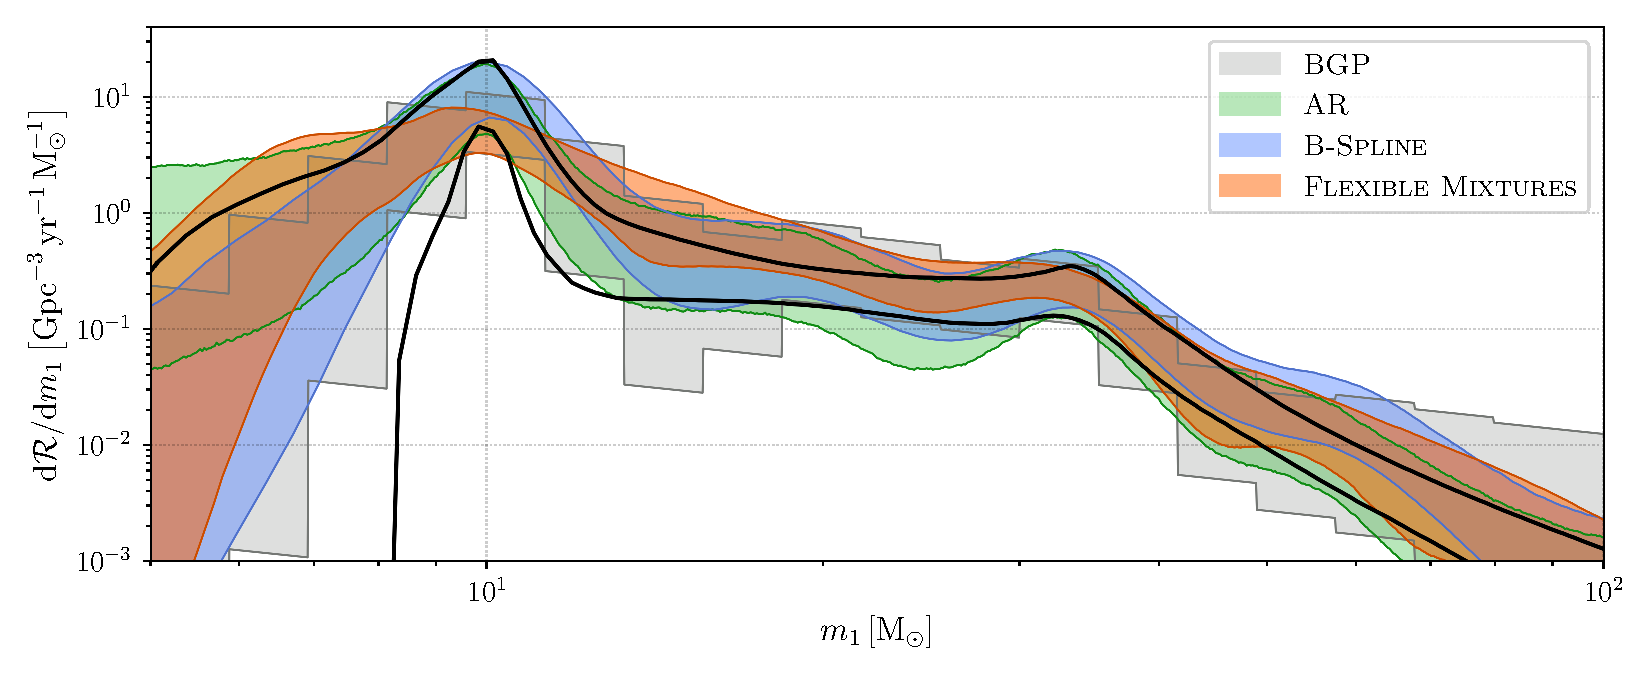
\includegraphics[width=\textwidth]{figures/primary_mass_non_parametric.pdf}
	  \includegraphics[scale=0.7]{figures/mass_ratio_non_parametric.pdf}
	  \caption{(\textit{Top}) Primary mass distributions using the \nonparametrics outlined in Appendix \ref{appendix:non_parametric_models_summary}. The \BrokenPLTwoPeaks result is shown in black for comparison. All distributions show rates evaluated at $z=0.2$, except for BGP, which shows the rate evaluated on the $z=0.1-0.25$ bin. Note that Flexible Mixtures does not infer primary mass directly, but instead derives it from the chirp mass Gaussian mixture model and the mass ratio as a power law distribution. The lack of substructure in the Flexible Mixtures mass distribution relative to the other models is likely due to model misspecification from assuming a power law mass ratio model. (\textit{Bottom}) Mass ratio distributions using the \nonparametrics outlined in Appendix \ref{appendix:non_parametric_models_summary}. The \BrokenPLTwoPeaks result is shown in black for comparison. Flexible Mixtures models the chirp mass as a Gaussian mixture model and the mass ratio as a power law. For the \BSpline and \ac{AR} models, the separable distribution $p(q)$ is shown by dashed lines and the conditional marginal distribution $p(q|m_2 > 3\Msun) = \int p(q)p(m_1)\Theta(m_1q-3){\rm d}m_1$ is shown by the shaded regions, highlighting that the low mass ratio truncation seen in the \parametric is largely a prior effect.}
	  \label{fig:bbh_mass_non_parametrics}
  \end{figure*}

\textit{Mass distributions}: We supplement the \parametric with various \nonparametrics. Figure \ref{fig:bbh_mass_non_parametrics} (top panel) shows the inferred primary mass distribution using the \BSpline, AR, Flexible Mixtures, and BGP models compared to the fiducial \BrokenPLTwoPeaks model. All models agree within their $90\%$ credible regions, though the Flexible Mixtures model is the only model that does not exhibit a prominent peak at ${\sim}10 \Msun$. The Flexible Mixtures model does not directly infer the primary mass, but instead it models the chirp mass as a Gaussian mixture model and the mass ratio with a power law. The primary mass distribution shown in Figure \ref{fig:bbh_mass_non_parametrics} is then derived from these two distributions. The discrepancy between this model and the other \nonparametrics could be due to model misspecification, i.e., assuming the mass ratio distribution follows a power law for all primary masses. The fact that the discrepancy exists primarily in the ${\sim}10 \Msun$ region supports the \textsc{Isolated Peak} result in Section \ref{subsec:bbh_ratio}, which suggests the ${\sim}10 \Msun$ peak disfavors equal mass mergers (i.e., is inconsistent with a power law in mass ratio) compared to higher mass \acp{BBH}. The mass ratio distributions inferred by the \BSpline, AR, and Flexible Mixtures is shown Figure \ref{fig:bbh_mass_non_parametrics} (bottom panel). The $90\%$ credible regions are consistent between each model. The \BSpline model infers a peak away from $q=1$, which is not present in the AR or Flexible Mixtures results. This may be due to the \BSpline model's greater flexibility compared to the AR and Flexible Mixtures models, as it infers all parameters simultaneously with B-Splines. The AR model assumes an auto-regressive process only in primary mass and mass ratio, while other parameters are inferred with the fiducial models listed in Table \ref{tab:summary_of_models}. As noted in Appendix \ref{appendix:BSpline}, the figure includes the marginal distributions conditioned on $m_2 > 3\Msun$ from the \BSpline and AR models in addition to the fully separable components (dashed lines). The two distributions are essentially identical above $q \sim0.4$, below which the marginal distribution falls off sharply. This implies that the behavior of the \parametric below $q \sim 0.4$ is primarily due to the prior assumption of a minimum mass cutoff, and not due to information inferred about the shape of the distribution in that regime. 

\textit{Effective spin distributions}: In addition to the \skewnormalChiEff model and various correlation models presented for $\chieff$ in the main text (Figures~\ref{fig:chi_eff_chi_p_pdf} and \ref{fig:q_chieff_ppd}), we use the \nonparametric for a consistency check and find the distributions shown in the top panel of Figure~\ref{fig:effective_spins_nonparametric}. 
We plot the $\chieff$ distribution directly inferred with a binned Gaussian process (BGP; blue) as well as that reconstructed from the spin magnitude and tilt \BSpline model results (green), and compare them to the \skewnormalChiEff (red-orange), \effectiveSpinModel (purple), and $(q,\chieff)$ \splinecorrelation (maroon) results from the main text. 
The two approaches paint the same qualitative picture: the $\chieff$ distribution peaks at small values.
However, there is variation between the \nonparametric and \parametric; the \nonparametricAdj distributions are wider than the \parametricAdj distributions.
In Figure~\ref{fig:effective_spins_nonparametric}, we additionally plot posteriors distributions on statistics derived from each $\chieff$ distribution (c.f., Table~\ref{tab:min_chieff}), with results summarized as follows:
%
\begin{itemize}
%
	\item \textit{First percentile of the $\chieff$ distribution} ($\chi_{\mathrm{eff}, 1\%}$): 
	The three \parametricAdj distributions find consistent first-percentiles, around $\sim 0.2$, while the \nonparametricAdj find that the $\chieff$ distribution extends to lower values. 
	In the case of the BGP, the first-percentile distribution rails against the minimum allowed value of $-0.7$. 
% 
	\item\textit{Fraction of \acp{BBH} with negative} $\chieff$: 
	All models yield consistent posteriors with one another and find that the fraction of \acp{BBH} with negative $\chieff$ is greater than zero and less than $\sim 0.8$. 
	The BGP posterior on this fraction is the widest, and the \BSpline posterior peaks at a higher values than the near-identical \parametricAdj posteriors.
% 
	\item \textit{HM fraction}:
	The HM fraction is a heuristic for the upper limit of the fraction of \acp{BBH} coming from hierarchical mergers; it is calculated as $1/0.16$ times the fraction of BBHs with $\chieff < -0.3$, based on the fact that $\sim 16\%$ of hierarchical mergers are theorized to have $\chieff < -0.3$~\citep{Fishbach:2022lzq,Baibhav:2020xdf}. 
	The different models yield a range of 90\% upper limits for the HM fraction.
    With the three parametric models, we consistently find the HM fraction to be small at $\lesssim 8\%$.
	The two more flexible non-parametric models, on the other hand, find support up to larger values of $27\%$ (\BSpline) or $74\%$ (BGP).
%
	\item \textit{Skew of the $\chieff$ distribution about its peak}: 
	Each model finds fairly different values of the skew, which is here defined as the difference between the fraction of $\chieff > \chi_0$ and $\chieff < \chi_0$, where $\chi_0$ is the value of $\chieff$ at which the distribution peaks~\citep[][Equation 5]{Banagiri:2025dxo}.
	By design, the \effectiveSpinModel~model will always have a skew of $\sim 0$: truncated normal distributions are approximately symmetric about their peak if the truncation occurs substantially far from the distribution's bulk, which is here the case.
	All other models find a preference for positive skew, meaning that the distribution has more support for $\chieff$ above its peak than below. 
	This is the most pronounced for the \skewnormalChiEff, which is entirely inconsistent with a skew of 0. 
%
\end{itemize}
%


%
\begin{figure}
	\centering
	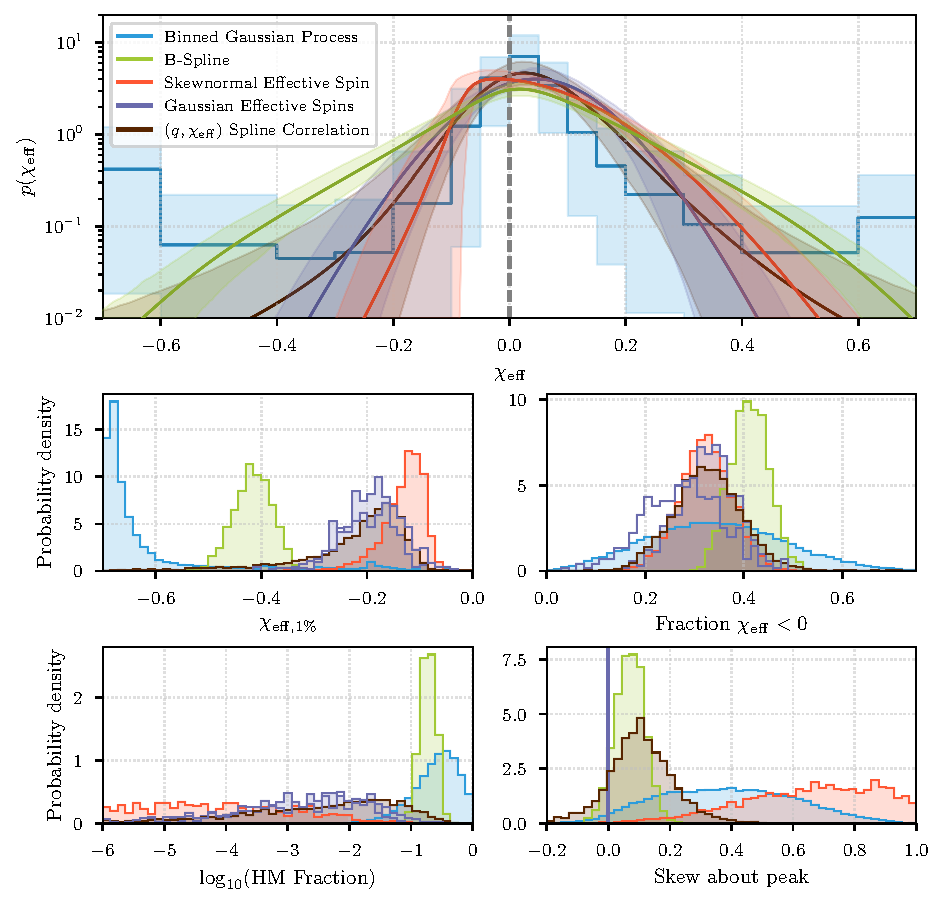
\includegraphics[width=0.9\linewidth]{figures/spins/chi_eff_traces_nonparametric.pdf}
	\caption{
		\textit{First row:} Marginal $\chieff$ distributions with BGP (blue) and \BSpline (green) models, as compared to the \skewnormalChiEff (red-orange), \effectiveSpinModel (purple), and $(q,\chieff)$ \splinecorrelation (maroon) models.
		The \ac{PPD} (average) is shown with a dark line, and the 90\% confidence intervals are shaded.
		\textit{Second and third rows:} Posteriors on the first percentile of the $\chieff$ distribution (upper left), the fraction of $\chieff<0$ (upper right),  HM fraction (lower left), and the skew (lower right).
		See Section~\ref{subsubsec:bbh_effective_spins} for a discussion of these quantities.
		Colors correspond to the top panel; purple dashed is \gwtcthree with the \effectiveSpinModel model for comparison.
	} 
	\label{fig:effective_spins_nonparametric}
  \end{figure}
%

\subsection{Merger Rates Including Subthreshold Triggers}\label{appendix:FGMC_rates}

Search pipelines compute \acp{SNR} of detector data to identify portions of 
data with above-threshold \ac{SNR}, i.e., ``triggers", which may contain 
\ac{GW} events~\citep{GWTC:Methods}.
Based on pipeline-specific ranking statistics, triggers are assigned 
significances quantified by \acp{FAR}. 
In the main text, merger rates were calculated from population analyses that 
only used triggers surpassing a fixed-significance \ac{FAR} threshold, which was 
motivated to introduce minimal contamination from noise events.
By design, the list of triggers included in those analyses is threshold-dependent. 
Here, we explore the merger rates by including subthreshold triggers 
~\citep{Farr:2013yna, Kapadia:2019uut}, which ensures that the inferred rates 
are free of biases due to arbitrary significance thresholds and mitigates loss 
of information from excluding subthreshold GW candidates.
Specifically, we consider the full set of available triggers from a 
matched-filtering search, 
\GSTLAL~\citep{Messick:2016aqy, Sachdev:2019vvd, Hanna:2019ezx, Cannon:2020qnf, Ewing:2023qqe, Tsukada:2023edh, Sakon:2022ibh, Ray:2023nhx, Joshi:2025nty, Joshi:2025zdu}. 

The method used by \GSTLAL to self-consistently classify triggers and compute 
$p_{\rm astro}$~\citep{LIGOScientific:2018mvr, LIGOScientific:2021usb, KAGRA:2021vkt, Kapadia:2019uut, GWTC:Methods, GWTC:Results, Ray:2023nhx} 
values provides the rate densities described here for \acp{BNS}, \acp{NSBH}, 
and \acp{BBH}~\citep{GWTC:Methods, Kapadia:2019uut}.
The approach is a simplified version of the methods described in Appendix C 3 of 
\citet{KAGRA:2021duu}, as well as the discovery of GW200105 and 
GW200115~\citep{LIGOScientific:2021qlt} and GW230529~\citep{LIGOScientific:2024elc}. 
The simplification involves fixing the mass distribution to the Salpeter 
model~\citep{Salpeter:1955it} as opposed to marginalizing over population 
uncertainties inferred by the above-threshold event analyses explored in the main 
text.
We do not expect the marginalization over population uncertainties to have a 
significant impact on the inferred merger rates, given the uncertainty ranges.
When we apply the simpler model to \gwtcthree~\citep{KAGRA:2021duu}, the estimated
rates are comparable to those derived when marginalizing over the inferred population.
For effective inspiral spins of each trigger, we use a uniform distribution. 
Consistent with how searches categorize triggers and compute 
\VT~\citep{GWTC:Methods}, we set the boundary between \acp{NS} and 
\acp{BH} to be $3~\Msun$. 
For triggers categorized as \ac{BNS} or \ac{NSBH}, we set the bounds of the 
spins corresponding to a \ac{NS} to $\pm 0.4$.
These bounds are consistent with what the analyses in the main text adopt 
(see Section~\ref{subsec:event_selection} and Section~\ref{sec:ns}).

Using the fixed population distribution and the Poisson mixture model of 
~\cite{Kapadia:2019uut}, we  infer the merger rate densities of the different 
source categories (\ac{BNS}, \ac{NSBH}, and \ac{BBH}) from the full list of 
available \GSTLAL triggers with \ac{FAR} $<$ $1$ $\text{hour}^{-1}$.
This is done while self-consistently accounting for the 
possibility that some of these triggers are likely noise artifacts. 
We construct the posterior of astrophysical counts of \ac{BNS}, \ac{NSBH}, 
and \ac{BBH} events by utilizing mass-based binning template weights~\citep{Ray:2023nhx}.
We estimate the time--volume sensitivity~\citep{Tiwari:2017ndi, GWTC:Methods} 
$\VT$ for each event category $\alpha$ 
($\alpha = $ \ac{BNS}, \ac{NSBH}, \ac{BBH}), using injections~\citep{Essick:2025zed}, 
and their contributions to the counts posterior~\citep{Kapadia:2019uut}. 
Finally, we compute the rates posterior from marginalized counts posterior and 
the estimated $\VT$~\citep{LIGOScientific:2018mvr, LIGOScientific:2020kqk, KAGRA:2021duu, GWTC:Results}:
\begin{equation}
	p\left(R_\alpha\right) = p\left(\Lambda_{1 \alpha} | \mathbf{x} \right) \VT_{\text{O1-O4a}, \alpha} .
	\label{eq:fgmc}
\end{equation}
Here, $p\left(\Lambda_{1 \alpha} | \mathbf{x} \right)$ is the marginalized counts 
posterior where $\Lambda_{1 \alpha}$ is the astrophysical count for event 
category $\alpha$ and 
$\Lambda_{1 \alpha} = R_\alpha \VT_{\text{O1-O4a}, \alpha}$.
Here, $\text{O1-O4a}$ indicates that data from \ac{O1} throughout \ac{O4a} are used. 
The vector $\mathbf{x}$ represents the set of triggers using in this analysis, 
where each $x_i$ consists of the ranking statistics information, \ac{SNR}, and 
an identifier for the template associated with the trigger.

A Jeffreys prior, $\propto N^{-1/2}$, is imposed on the astrophysical counts 
for \acp{BBH} to construct their posterior from the mixed Poisson likelihood 
and compute the merger rate. 
The merger rate of \acp{BBH} is computed to be 
$\CIBoundsDash{\FgmcRates[RatesBBH]}$ $\perGpcyr$. 
This is consistent with the \ac{BBH} merger 
rate provided in the analyses presented in the main text, and the rate has been 
further narrowed compared to the results of \citet{KAGRA:2021duu} while still 
being consistent within uncertainties.  
A uniform prior is used for \acp{NSBH} and \acp{BNS}, as the number of detected 
events containing a \ac{NS} is small. 
We compute the \ac{NSBH} merger rates to be 
$\CIBoundsDash{\FgmcRates[RatesNSBH]}$ $\perGpcyr$, 
which is consistent with the \ac{NSBH} merger rate presented in main text. 
Similarly to the rate for \acp{BBH}, the rate of \acp{NSBH} is consistent with 
the rate obtained from the analyses of \gwtcthree but has been further narrowed.
The \ac{BNS} merger rate is calculated to be 
$\CIBoundsDash{\FgmcRates[RatesBNS]}$ $\perGpcyr$, 
which is consistent with the \ac{BNS} merger rate presented in the main text and 
has been narrowed down compared to the rate obtained from the analyses of 
\gwtcthree.

\subsection{Supplementary Results: BBH Correlations}\label{appendix:supplementary_correlations}

Here, we supplement the correlated \ac{BBH} population results presented in Section~\ref{sec:Population-level correlations between parameters} with additional results and figures.
In the top panel of Figure~\ref{fig:correlation_appendix}, we plot the posterior distribution for the level of correlation $\kappa_{\chieff, z}$ inferred in the \copulacorrelation~model for $(z,\chieff)$.
Note the peak at positive values, and long tail into negative values.
The middle panels show the inferred mass distributions, using a mass-redshift correlated \ac{BGP}~analysis, binned by redshift.
We see that both the primary and secondary mass distribution appear to be broadly consistent across redshifts up to $z = 1$.
Finally, we investigate mass and spin correlations with the data-driven \vamana~analyses.
In the bottom panels of Figure~\ref{fig:correlation_appendix}, we plot the inferred distribution of orbital aligned spin $\chi_z$ as a function of both chirp mass and mass ratio, obtained with the \vamana~analysis.
We see that the results have a large degree of uncertainty, and are broadly consistent with findings explored here and in Section~\ref{sec:Population-level correlations between parameters}.

\begin{figure*}
	\centering
	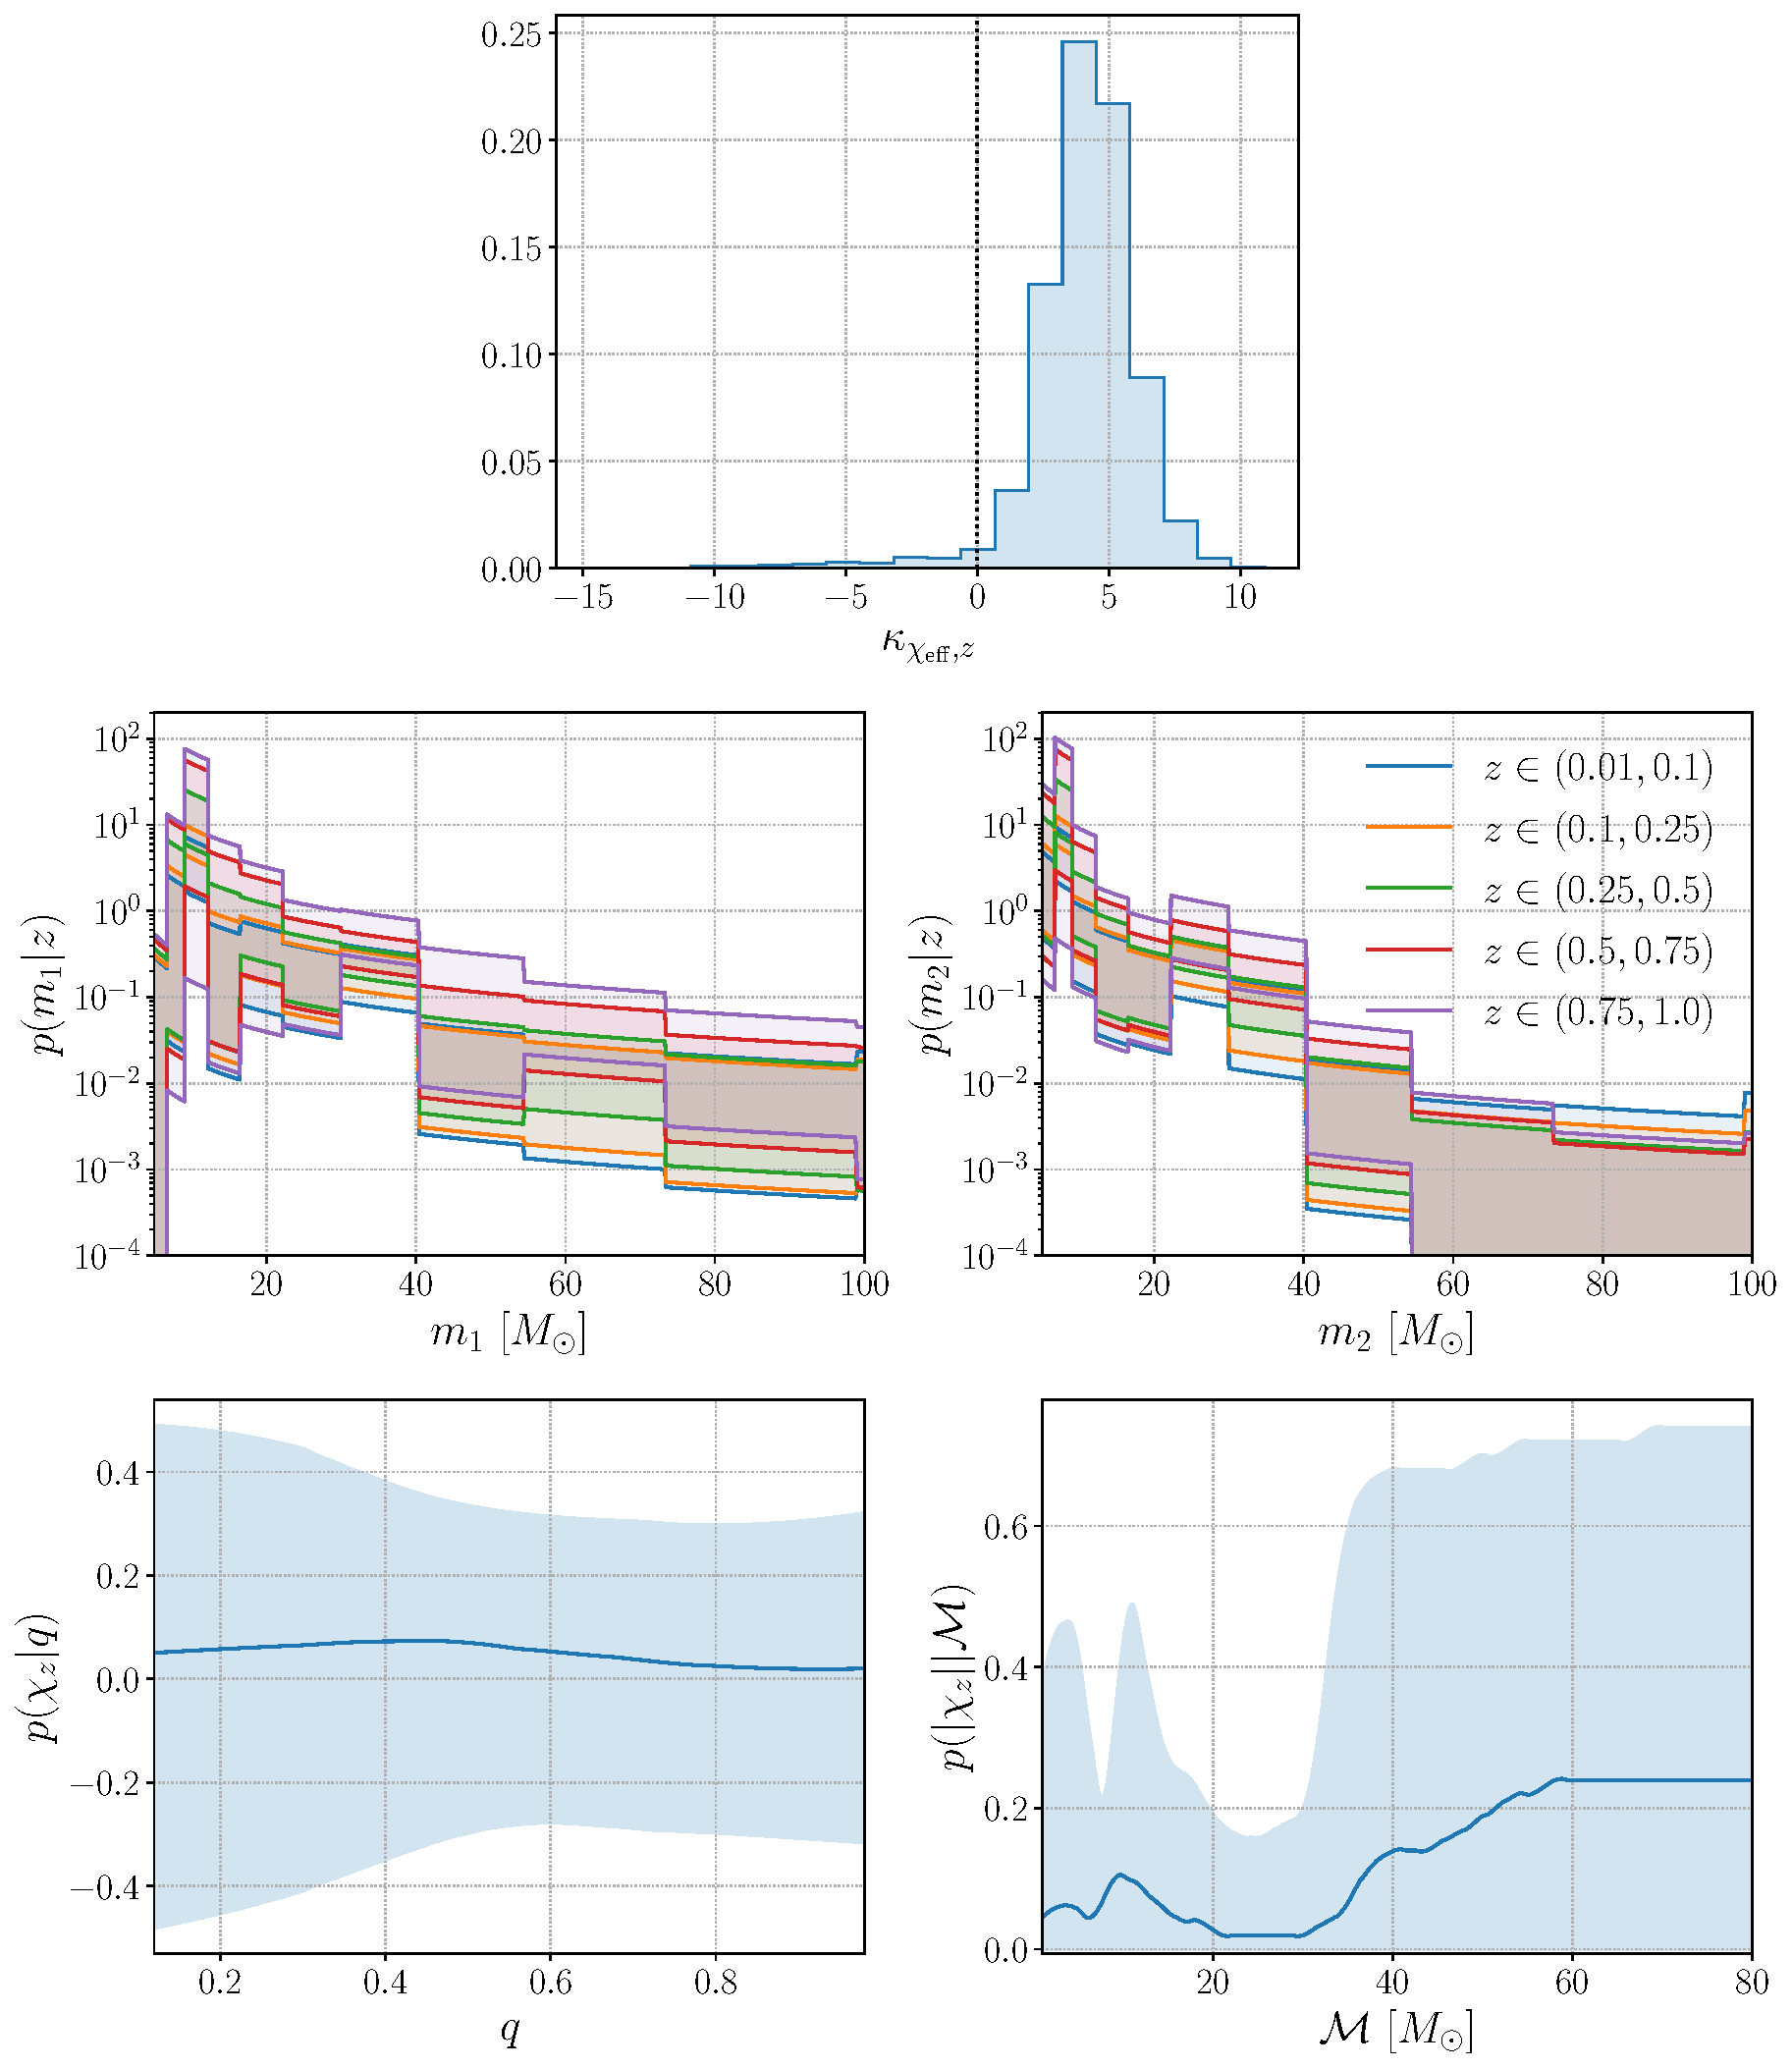
\includegraphics[width=0.9\columnwidth]{figures/correlation_appendix.pdf}
	\caption{
	\textit{Top:} Posterior distributions for the level of correlation between redshift and effective inspiral spin $\kappa_{\chieff, z}$ inferred using the \copulacorrelation~model.
	The vertical black dashed line in each plot indicates a value of $\kappa_{\chieff, z}$, at which no correlation is implied.
	\textit{Middle:} Inferred distributions of primary mass (left), and secondary mass (right) in the redshift and spin correlated \ac{BGP}~analysis.
	The solid lines bound the \confidenceLevel~credible intervals for each redshift bin.
	We can see that all redshift bins from $z=0.01$ to $z=1$ are consistent within \confidenceLevel~credibility.
	\textit{Bottom:} Correlated mass and spin \acp{PPD} from the \vamana~model.
	Solid lines give the medians, while the shaded regions encompass 90\% of the \ac{PPD} volume.
	The left panel gives the inferred distribution of aligned spin $\chi_z$ given mass ratio.
	We do not see any evidence for or against a correlation.
	The right panel gives the inferred distribution of the aligned spin magnitude $|\chi_z|$ as a function of chirp mass.
	We see that the uncertainty is very large, with a notable drop in the ${\sim} 20{-}30 \,\Msun$ region.
	For reference, this region very roughly corresponds to the $30 \,\Msun$ peak observed in the component mass distributions (a $30 \,\Msun + 30 \,\Msun$ \ac{BBH} has a chirp mass of $\mathcal{M} \approx 26 \,\Msun$).
	Following the mass- and spin-correlated \ac{BGP} results then, it is unsurprising that the \vamana results prefer a local minimum in aligned spin magnitude in this region.
	}
	\label{fig:correlation_appendix}
\end{figure*}
